\documentclass[10pt,conference]{IEEEtran}
\IEEEoverridecommandlockouts
\usepackage{cite}
\usepackage{amsmath,amssymb,amsfonts}
\usepackage{graphicx}
\usepackage{booktabs}
\usepackage{array}
\usepackage{url}
\usepackage{microtype}
\graphicspath{{artifacts/}}

\begin{document}

\title{Green by Default? A Deployed Energy-Saving LLM Router\\Uses More Energy than Ignoring the Query}

\author{\IEEEauthorblockN{Anonymous Author(s)}
\IEEEauthorblockA{\textit{Anonymous Institution}\\
anonymous@example.com}
\thanks{Submitted to the 11th International Workshop on Green and Sustainable Software (GREENS 2027), co-located with ICSE 2027. Single-anonymous review.}}

\maketitle

\begin{abstract}
Systems that route questions among large language models (LLMs) increasingly advertise energy savings relative to a ChatGPT-style default: send every query to a frontier model. That comparison is nearly uninformative. Any policy that rarely calls the frontier will ``save'' energy, including the query-independent constants ``always use the small model'' and ``always use the middle model.'' The sustainability question is whether a router reduces energy versus the cheapest \emph{competent} static policy on the same workload.

We study EcoLogic, a deployed three-tier Q\&A router that reports joules saved using assumed rates of $0.5$, $1.5$, and $60$\,J per 1k tokens. \textbf{No joule was metered}: energy is a linear transform of provider token counts. On $364$ objectively graded items, the advertised router uses $689$\,J at $86.8\%$ accuracy. The constant policy Always-Tier-2 uses $394$\,J---$0.57\times$ the router's modelled energy---at $92.3\%$ accuracy ($+5.5$\,pp; McNemar $p=3.2\times10^{-4}$, Holm $p=9.7\times10^{-4}$). That ranking survives a $21$-cell mix simplex, leave-one-benchmark-out, and a $10{,}000$-item bootstrap ($99.99\%$), and it holds in tokens ($4.42\times$) before any joule rate is applied. Always-frontier uses $6066$\,J at $91.5\%$. The router's headline $88.6\%$ modelled-joule saving versus the frontier is therefore a reporting artifact of the baseline: the same decisions save only $55.0\%$ in measured USD. A $\pm5\times$ factorial over the three rates ($27$ cells) shows that the versus-frontier saving ranges from $-165\%$ to $+99\%$ and \emph{flips sign in $3/27$ cells}. Versus Always-Tier-2, the router uses more modelled energy in $19/27$ cells.

When a middle tier already dominates quality and energy, query-conditioned escalation is a green-architecture anti-pattern: extra energy, extra frontier calls, and no quality gain. Green software metrics that treat always-frontier as the default comparator can be gamed. We argue for static single-tier controls and explicit energy-model sensitivity as first-class reporting requirements---and we bound every joule claim by the unmetered linear model that produced it.
\end{abstract}

\begin{IEEEkeywords}
Green software engineering, Green AI, energy metrics, LLM inference, software architecture, sustainability reporting
\end{IEEEkeywords}

\section{Introduction}

EcoLogic is a deployed three-tier LLM router whose API returns not only an answer but a quantity named \texttt{energy\_saved}. That quantity is computed by comparing the tokens consumed on the chosen tier against a hypothetical frontier call priced at $500$\,J per 1k tokens---a GPT-5 default that the serving stack never actually ran. Even under the milder comparison used in the system's evaluation write-up (always \texttt{gpt-4o} at $60$\,J/1k), the marketing claim is of the form ``we saved $\sim$89\% of the energy of ChatGPT.'' Green software engineering has spent a decade warning that such savings claims are only as good as the baseline, the metric, and the measurement apparatus~\cite{naumann2011greensoft,lago2015framing,schwartz2020green,calero2021green}. This paper takes that warning literally for LLM routing.

A tiered router sends apparently easy queries to a small model and apparently hard ones to a larger model, then reports the energy it avoided relative to sending everything to the frontier. The comparison is the field's standard one, and it is nearly uninformative, because \emph{it is not the bar the router has to clear}. Two much cheaper policies also beat always-frontier on energy: always use the small model, and always use the middle model. Neither inspects the query. A router earns its complexity, from a sustainability standpoint, only if it beats \emph{those}.

The research question is therefore not ``does the router save energy versus the frontier?''---it will, trivially, under any rate vector that makes the frontier expensive per token---but:

\begin{quote}
\emph{Do systems that advertise energy-saving LLM routing reduce modelled energy versus the cheapest competent static policy, and is that conclusion robust when the energy-rate model is varied?}
\end{quote}

We answer on one deployed system, EcoLogic, using committed generations (no new API calls). The study object is a keyword classifier over three substituted models (Qwen3.5-9B, \texttt{gpt-oss-20b}, \texttt{gpt-4o}) on $364$ auto-graded items (HumanEval, MMLU, GSM8K)~\cite{chen2021evaluating,hendrycks2021mmlu,cobbe2021gsm8k}. Energy is
\[
E(\pi)=\sum_{x}\frac{\mathrm{tokens}(x,\pi(x))}{1000}\,r_{\pi(x)},
\]
with EcoLogic's own assumed rates $r=(0.5,1.5,60)$\,J per 1k tokens. Token counts are real provider \texttt{usage} fields. The rates are not. We treat that fact as the primary threat to validity, not a footnote, and we promote a $\pm5\times$ per-tier factorial over $r$ to a first-class experiment.

\textbf{Findings.} Under the paper rates, Always-Tier-2 Pareto-dominates EcoLogic on the energy--accuracy plane: $+5.5$ percentage points (pp) accuracy at $0.57\times$ the modelled joules (Table~\ref{tab:energy}). The advertised $88.6\%$ joule saving versus always-frontier shrinks to $55.0\%$ when the identical assignments are priced in measured USD---a green-measurement result: the choice of cost model moves the residual by a factor of four (Table~\ref{tab:axes}). The versus-frontier saving is not even sign-stable under $\pm5\times$ rate error (Fig.~\ref{fig:sens}). Architecturally, the middle tier already dominates both quality and energy on this workload; adding a query-conditioned router then \emph{increases} modelled energy while \emph{decreasing} accuracy. That is a sustainability anti-pattern, not a green default.

We claim no physical energy measurement, no result about routers in general, and no success for the $88\%$ headline. The contribution is a negative case study plus a reporting prescription for green software metrics applied to generative-AI systems. Concretely: (1)~an energy$\times$accuracy table in which the advertised router is Pareto-dominated by a query-independent constant; (2)~a $\pm5\times$ factorial that is treated as an experiment on the energy model, including the Always-T2 ranking that the versus-frontier literature omits; (3)~a per-benchmark energy mix; (4)~the joules-versus-dollars gap as evidence that cost-model choice is itself a sustainability-reporting failure; and (5)~an architectural reading---query-conditioned three-tier routing as an anti-pattern when the middle tier already dominates.

This is an emerging-research workshop paper: one system, one substituted stack, one academic mix. Its value for GREENS is the metric and architecture argument, which can be reused on any $k$-tier LLM serving design, not the claim that ``routing does not work.''

\section{Background}

\subsection{Green software and Green AI}

Green software engineering treats energy and other sustainability dimensions as first-class quality attributes of software-intensive systems~\cite{naumann2011greensoft,lago2015framing,calero2015green,calero2021green}. Architectural work has long argued that distribution choices, deployment topology, and design tactics dominate runtime energy once algorithms are fixed~\cite{procaccianti2015green,jagroep2017energy,capilla2024architecture,cruz2021energy}. GREENS 2027 explicitly solicits metrics that cannot be gamed, architectural anti-patterns, and Green AI for generative systems.

Machine-learning energy research split early into \emph{Red AI} (accuracy at any compute) versus \emph{Green AI} (efficiency as a reported result)~\cite{schwartz2020green}. Training-time carbon accounting for large models~\cite{strubell2019energy,patterson2021carbon,luccioni2023bloom,wu2022sustainable,faiz2024llmcarbon} established that assumed grid intensity, hardware utilisation, and system boundaries move headline tonnes as much as model size does. Strubell et al.'s widely cited training-cost estimates were themselves scenario calculations, not rack-level traces~\cite{strubell2019energy}; subsequent work showed that cloud-instance carbon intensity varies by region and time of day~\cite{dodge2022measuring}. Inference, not training, now dominates the operational footprint of deployed LLMs~\cite{luccioni2024power,samsi2023words}. Samsi et al.\ \emph{did} meter watts on LLM inference; Luccioni et al.\ showed that deployment-time energy can dwarf training when a model is served at scale. Surveys of Green AI in software engineering document both a rapid growth of papers and a persistent measurement gap: many studies report proxy metrics (FLOPs, parameters, tokens, cloud invoices) rather than joules~\cite{verdecchia2023green,martinez2022green,bannour2021evaluating,henderson2020towards}. This paper sits in that gap. We do not close it with a wattmeter. We show what happens when a deployed system treats a token-linear proxy as if it were energy, and when the baseline is the most expensive policy in the set.

Two further SE observations shape the design. First, energy is an architectural property: Jagroep et al.\ argued for extending architecture views with consumption, and Procaccianti et al.\ found that cloud software-architecture decisions dominate once algorithms are fixed~\cite{jagroep2017energy,procaccianti2015green}. A router is such a decision---an extra control element in the path. Second, sustainability reporting can be gamed by the choice of functional unit~\cite{lago2015framing,calero2021green}. ``Energy per ChatGPT-equivalent query'' is a functional unit that makes any cheaper model look green. ``Energy per correct answer versus the cheapest competent model'' is a stricter unit. We use the latter.

\subsection{LLM routing as an energy tactic}

Routing and cascading---FrugalGPT, RouteLLM, hybrid LLM routers---aim to preserve quality while sending easy queries to cheaper models~\cite{chen2023frugalgpt,ong2025routellm,stoica2024router}. Cost is almost always dollars or call fraction. Energy, when reported, is typically a restatement of tokens times an assumed intensity. The green-SE question is whether the \emph{architecture} (a query-conditioned dispatcher in front of a heterogeneous model pool) is an energy tactic or an energy anti-pattern. That depends on whether any static member of the pool already dominates the Pareto front. If it does, the dispatcher is pure overhead plus mis-routing.

\section{Study Object}

\subsection{The deployed router}

EcoLogic classifies each prompt with a local keyword/heuristic function (\texttt{classify\_prompt\_local\_nlp}) into one of three tiers. The classifier is not a learned model and is not a billed API call. Production slugs were Gemma~3N~E4B (Tier~1) and Apriel~1.6~15B (Tier~2) on Together AI, plus \texttt{gpt-4o} (Tier~3). Those Together slugs were retired before this evaluation; we used energy-adjacent substitutes Qwen3.5-9B and \texttt{gpt-oss-20b}. The routing \emph{logic} is the production function; the model \emph{stack} is not. Both substitutes are reasoning models that emit long traces, which the retired models did not. Token inflation relative to \texttt{gpt-4o} is therefore likely an artifact of substitution (Section~\ref{sec:threats}).

\subsection{Assumed energy model}

Rates hard-coded in the serving application are $r_1=0.5$, $r_2=1.5$, $r_3=60$\,J per 1k tokens, with a still more extreme GPT-5 comparator at $500$\,J/1k used to populate \texttt{energy\_saved}. The product formula is
\[
\texttt{energy\_saved}=\max\bigl(0,\; \tfrac{\mathrm{tokens}}{1000}\cdot 500 - \tfrac{\mathrm{tokens}}{1000}\cdot r_{\mathrm{chosen}}\bigr),
\]
i.e., it prices a ghost frontier call at the \emph{same token count} as the cheap model. That is not a counterfactual of ``what gpt-4o would have spent on this query'' (gpt-4o uses far fewer tokens) and not a wattmeter reading. We evaluate the $0.5/1.5/60$ vector because it is the one attached to the three tiers that actually ran, and we separately price assignments in USD. Energy of a policy $\pi$ is the sum in Section~I. Equivalently, if $T_t(\pi)$ is the total tokens assigned to tier $t$,
\[
E(\pi)=\sum_{t\in\{1,2,3\}} T_t(\pi)\cdot r_t/1000.
\]
This is a \emph{linear transform of token counts under assumed rates}. It does not include prompt-processing versus generation split, batching, utilisation, idle draw, PUE, cooling, or the classifier's CPU energy (the last is negligible next to LLM calls, but unmeasured). Provider APIs expose tokens, not watts. Throughout, ``energy'' means this model. We never write that a joule was observed.

\subsection{What is measured}

Item-level fields from $1{,}092$ graded calls ($364$ items $\times$ $3$ tiers), temperature~$0$: \texttt{total\_tokens}, \texttt{usd} from provider usage, and an objective grade (HumanEval by execution of the official tests; MMLU by letter match; GSM8K by final-number match). No LLM-as-judge. Completeness: $0$ missing tier-item pairs, so every comparison is paired.

\section{Method}

\subsection{Static policies as sustainability controls}

On the identical $364$-item set we evaluate:
\begin{itemize}
\item \textbf{EcoLogic}: the production classifier on the raw user query (the input a user types; wrapped benchmark instructions agree with raw routing on only $53\%$ of items, and we report the user-facing choice).
\item \textbf{Always-T1} / \textbf{Always-T2} / \textbf{Always-frontier}: query-independent constants. Always-T2 is the cheapest competent static policy \emph{ex post} on this mix; we do not pretend it was chosen before seeing the data, and we treat it as the control a green evaluation must include, not as a deployed default discovered for free.
\item \textbf{Random}: uniform tier per item, seed $20260905$, a sanity floor.
\item \textbf{Oracle}: per item, the lowest-energy tier that was actually correct under the rate vector in force; if none were correct, the cheapest response. An information-theoretic ceiling, not a deployable policy.
\end{itemize}
Accuracy uses Wilson score $95\%$ intervals~\cite{wilson1927}. Paired policy comparisons use McNemar's exact test~\cite{mcnemar1947}.

\subsection{Sensitivity design}

Let $m_t\in\{0.2,1,5\}$ scale each paper rate independently ($3^3=27$ cells, a $\pm5\times$ band). For each cell we recompute $E(\pi)$ from the \emph{same} token vectors---no regeneration---under $r'_t=m_t r_t$. Oracle assignment is recomputed because ``cheapest correct'' depends on $r$. We record (i)~EcoLogic's saving versus always-frontier, whose sign is the usual headline, and (ii)~EcoLogic's saving versus Always-T2, which is the green-SE comparison. A one-at-a-time tornado ($m_t\in\{0.2,5\}$, others at $1$) decomposes which rate moves the Always-T2 gap. The original evaluation corpus already tabulated the versus-frontier $27$-cell sweep; we reconstruct it from item-level tokens and add the Always-T2 ranking as this paper's additional axis.

The band is deliberately coarse. A $5\times$ error on an unsourced constant is not conservative in the sense of a statistical confidence interval; it is the smallest factor that, combined with the $11.5\times$ token inflation, can arithmetically reverse the versus-frontier margin ($\approx 10\times$ at paper rates). If a reviewer believes the rates are known to $2\times$, they may discard the three sign-flip cells and still cannot discard Always-T2's dominance under paper rates.

A second rate vector ($1.1/2.0/60$), committed as ``substitute-model rates,'' re-rates Tiers~1--2 upward because the models actually called are larger than the retired slugs. We report it as a structured alternative, not as a measurement.

\subsection{Joules versus dollars}

USD is summed from stored per-call \texttt{usd} fields (published \$/1M prices applied to prompt and completion tokens). No energy rate enters. The pair (modelled $E$, measured \$) on identical assignments is a measurement-method contrast: if they disagree about how large a ``saving'' is, the energy model is not a harmless unit change.

All tables and figures in Section~V are produced by \texttt{papers/greens/analysis.py} from \texttt{raw\_results/graded.jsonl} and \texttt{routing.json}. Frozen trees were not modified. Reconstruction matches committed \texttt{raw\_results/analysis.json} energy totals to floating-point precision ($688.953$\,J, $393.8595$\,J, $6065.88$\,J).

\section{Results}

\subsection{Energy $\times$ accuracy}

Table~\ref{tab:energy} and Fig.~\ref{fig:ea} are the primary result. EcoLogic reaches $86.8\%$ [$82.9\%$, $89.9\%$] at $689$\,J. Always-T2 reaches $92.3\%$ [$89.1\%$, $94.6\%$] at $394$\,J. The constant is $5.5$\,pp more accurate (McNemar $5$ vs.\ $25$ discordant items, $p=3.2\times10^{-4}$) at $394/689\approx0.57\times$ the router's modelled energy---equivalently, the router uses $1.75\times$ more energy than ignoring the query and sending everything to Tier~2. Always-T1 is statistically indistinguishable from EcoLogic on quality ($87.6\%$, McNemar $p=0.25$) and slightly cheaper ($677$\,J). Always-frontier is more accurate than EcoLogic ($91.5\%$, $p=9.5\times10^{-3}$) at $6066$\,J, $8.8\times$ the router and $15.4\times$ Always-T2. Oracle sits at $96.4\%$ / $386$\,J: the three-tier \emph{pool} has headroom; the classifier captures none of it.

\begin{table}[t]
\caption{Policies on $n=364$. Energy $=$ tokens/1000 $\times$ $0.5/1.5/60$\,J/1k; \textbf{not metered}. Wilson $95\%$ CIs. Mix $=$ T1/T2/T3.}
\label{tab:energy}
\centering
\setlength{\tabcolsep}{2.6pt}
\begin{tabular}{lrrrr}
\toprule
Policy & Acc.\ [CI] & J & vs T3 & Mix \\
\midrule
EcoLogic & 86.8 [82.9, 89.9] & 689 & 0.114$\times$ & 274/87/3 \\
Always-T2 & \textbf{92.3} [89.1, 94.6] & \textbf{394} & 0.065$\times$ & 0/364/0 \\
Always-T1 & 87.6 [83.9, 90.6] & 677 & 0.112$\times$ & 364/0/0 \\
Always-frontier & 91.5 [88.2, 93.9] & 6066 & 1.000$\times$ & 0/0/364 \\
Random & 90.7 [87.2, 93.2] & 2556 & 0.421$\times$ & 125/107/132 \\
Oracle & 96.4 [94.0, 97.9] & 386 & 0.064$\times$ & 160/194/10 \\
\bottomrule
\end{tabular}
\end{table}

\begin{figure}[t]
\centering
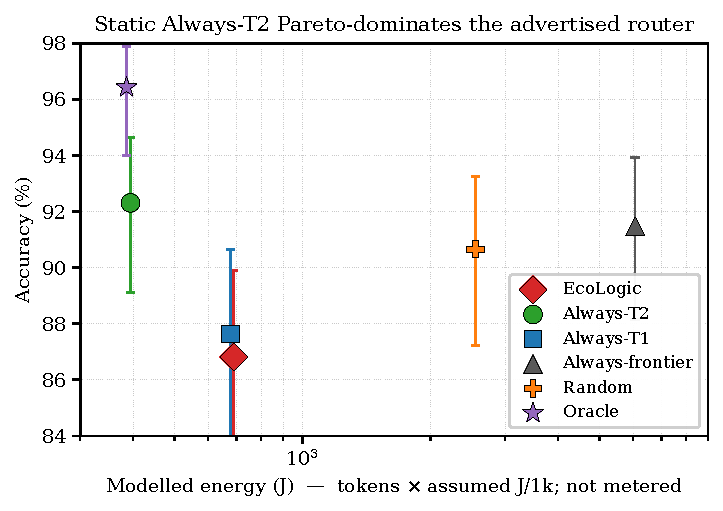
\includegraphics[width=\columnwidth]{fig_energy_accuracy.pdf}
\caption{Energy--accuracy plane under the token-linear model (log $x$-axis). Vertical bars are Wilson $95\%$ CIs. Always-T2 (circle) Pareto-dominates EcoLogic (diamond). Always-frontier sits far to the right at similar accuracy to Always-T2. Energy is modelled, not metered.}
\label{fig:ea}
\end{figure}

The mix explains the mechanism. EcoLogic sends $274/364$ items ($75\%$) to Tier~1, $87$ to Tier~2, and only $3$ to \texttt{gpt-4o}. Those $274$ Tier~1 calls consume $1{,}101{,}360$ tokens and $551$\,J---$80\%$ of the router's modelled energy---because the substitute small model is a verbose reasoner (system-wide EcoLogic tokens $1{,}161{,}679$ versus $101{,}098$ for always-\texttt{gpt-4o}: $11.5\times$ more tokens). The $88.6\%$ ``saving'' versus frontier is not less work; it is a $120\times$ assumed per-token advantage ($60/0.5$) only partly eaten by an $11.5\times$ token penalty. Three frontier calls still add $49$\,J. Always-T2 uses $262{,}573$ tokens. Escalation did not buy quality: of $90$ items EcoLogic moved off Tier~1, $0$ rescued a Tier~1 error and $3$ broke a Tier~1 success.

A production researcher degree of freedom is the prompt \emph{surface}. Feeding the classifier the wrapped benchmark instruction rather than the raw user query agrees on only $53.0\%$ of items, sends $174/364$ queries to \texttt{gpt-4o} (mix $137/53/174$), and multiplies modelled energy from $689$\,J to $3419$\,J at $89.6\%$ accuracy. We report the raw surface because that is what a user types and because it is the cheaper of the two EcoLogic variants. Surface choice moves the advertised joule total by $5.0\times$; it does not rescue domination by Always-T2.

Tier quality is not monotonic in advertised size. On HumanEval, Tier~2 scores $96.3\%$ versus $91.5\%$ for \texttt{gpt-4o} and $86.0\%$ for Tier~1. Overall, Tier~2 versus Tier~3 is not significant (McNemar $p=0.71$). There is no quality justification on this mix for paying the frontier rate.

Table~\ref{tab:tokens} decomposes tokens. EcoLogic's energy is $80\%$ Tier~1 ($551$\,J), $13\%$ Tier~2 ($89$\,J), and $7\%$ three frontier calls ($49$\,J). The ``green'' router is, under its own model, mostly a verbose small-model policy with a trickle of expensive calls.

\begin{table}[t]
\caption{Token volumes (provider \texttt{total\_tokens}) under paper-rate policies. EcoLogic does $11.5\times$ more token work than always-\texttt{gpt-4o}.}
\label{tab:tokens}
\centering
\begin{tabular}{lrrr}
\toprule
Policy & Tokens & J at paper $r$ & J / 1k tok \\
\midrule
EcoLogic & $1{,}161{,}679$ & $689$ & $0.59$ \\
Always-T2 & $262{,}573$ & $394$ & $1.50$ \\
Always-T1 & $1{,}354{,}186$ & $677$ & $0.50$ \\
Frontier & $101{,}098$ & $6066$ & $60.00$ \\
\bottomrule
\end{tabular}
\end{table}

\subsection{Per-benchmark energy mix}

Table~\ref{tab:bench} reconstructs modelled energy by benchmark. Always-T2 is cheaper than EcoLogic on every slice: HumanEval $220$ vs.\ $352$\,J, MMLU $76$ vs.\ $161$\,J, GSM8K $97$ vs.\ $175$\,J. The router's extra joules are not isolated to ``hard'' code. They are the global cost of preferring a verbose cheap-rate tier.

A rate-free check agrees. EcoLogic emits $4.42\times$ as many tokens as Always-T2 ($1{,}161{,}679$ vs.\ $262{,}573$). Table~\ref{tab:robust} collects the mix, leave-one-benchmark, bootstrap, and token-rank tests: none recovers the router. Modelled joules per correct answer are $2.18$\,J (EcoLogic) versus $1.17$\,J (Always-T2) versus $18.2$\,J (frontier). Holm-adjusted McNemar versus Always-T2 remains $p=9.7\times 10^{-4}$. The versus-frontier $88.6\%$ headline can be gamed; the versus-Always-T2 ranking cannot be recovered by mix reweighting or by dropping any one benchmark. Always-frontier's joules concentrate where \texttt{gpt-4o} emits more tokens (HumanEval $2895$\,J, GSM8K $2295$\,J, MMLU $876$\,J); the $88.6\%$ system-level saving versus frontier is therefore also a statement about how little work the frontier did per item relative to reasoning traces, not about routing skill. Fig.~\ref{fig:bench} shows the same mix as stacked bars.

\begin{table}[t]
\caption{Robustness of Always-T2 versus EcoLogic on modelled energy. None of these tests uses a new generation.}
\label{tab:robust}
\centering
\setlength{\tabcolsep}{3pt}
\begin{tabular}{lp{0.58\columnwidth}}
\toprule
Test & Result \\
\midrule
$21$-cell mix simplex & T2 cheaper in $21/21$ cells on J \emph{and} on tokens \\
Leave-one-benchmark ($7$) & T2 dominates accuracy and energy on all $7$ \\
Item bootstrap ($10$k) & T2 dominates in $99.99\%$ of draws \\
Token rank (rate-free) & EcoLogic emits $4.42\times$ T2's tokens \\
\bottomrule
\end{tabular}
\end{table}

\begin{figure}[t]
\centering
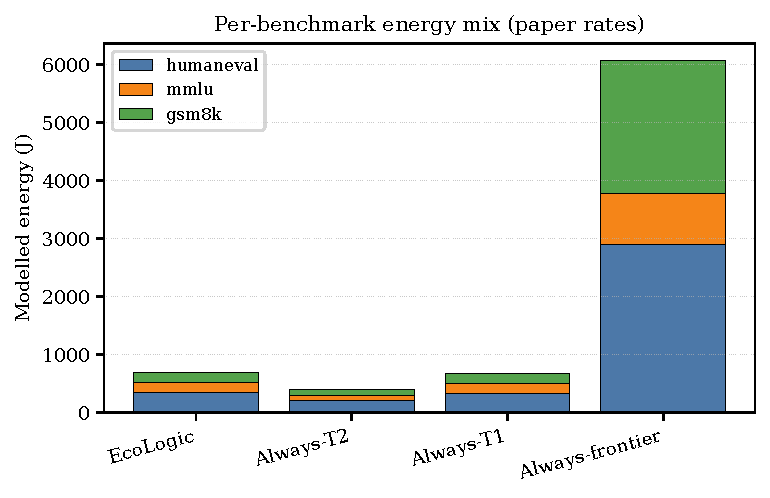
\includegraphics[width=\columnwidth]{fig_per_benchmark.pdf}
\caption{Per-benchmark modelled energy at paper rates. Always-T2 (second bar) is below EcoLogic on every colour (HumanEval, MMLU, GSM8K). Always-frontier's bar is dominated by HumanEval and GSM8K token volume priced at $60$\,J/1k.}
\label{fig:bench}
\end{figure}

\begin{table}[t]
\caption{Modelled energy (J) and accuracy by benchmark. Paper rates. EcoLogic is strictly more expensive than Always-T2 on every benchmark.}
\label{tab:bench}
\centering
\setlength{\tabcolsep}{3.5pt}
\begin{tabular}{lrrr}
\toprule
 & HumanEval ($n=164$) & MMLU ($100$) & GSM8K ($100$) \\
\midrule
EcoLogic & $352$\,J / $85.4\%$ & $161$ / $83\%$ & $175$ / $93\%$ \\
Always-T2 & $220$\,J / $96.3\%$ & $76$ / $84\%$ & $97$ / $94\%$ \\
Always-T1 & $333$\,J / $86.0\%$ & $173$ / $83\%$ & $171$ / $95\%$ \\
Frontier & $2895$\,J / $91.5\%$ & $876$ / $88\%$ & $2295$ / $95\%$ \\
\bottomrule
\end{tabular}
\end{table}

\subsection{Rate sensitivity as a first-class experiment}

Fig.~\ref{fig:sens} and Table~\ref{tab:sens} summarise the $27$-cell factorial. Versus always-frontier, EcoLogic's modelled saving ranges from $-164.6\%$ to $+98.8\%$. The sign flips in exactly three cells: all have $m_1=5$ (small-model rate understated by $5\times$) and $m_3=0.2$ (frontier rate overstated by $5\times$). That is a $25\times$ adverse swing against a $\sim$10$\times$ paper-rate margin, so reversal is arithmetic rather than exotic. It is also the direction one should worry about: $0.5$\,J/1k is an unsourced estimate for a \emph{retired} 4B-class model, and $60$\,J/1k for \texttt{gpt-4o} is equally unsourced.

Versus Always-T2, the router uses \emph{more} modelled energy in $19/27$ cells and less in $8/27$. The eight wins are exactly the cells with $(m_1,m_2)\in\{(0.2,1),(0.2,5),(1,5)\}$---i.e., when Tier~1 is cheap relative to Tier~2. No cell with $m_1=5$ favours the router over Always-T2. No cell with $m_2=0.2$ does either. Under EcoLogic's own paper rates $(1,1,1)$, and under the substitute-model rates $1.1/2.0/60$ (EcoLogic $1380$\,J vs.\ Always-T2 $525$\,J), the router remains the more expensive policy. The green-SE comparison is more stable than the versus-frontier headline: Always-T2 dominates on energy in the majority of the $\pm5\times$ cube \emph{and} on accuracy in every cell (accuracy does not depend on $r$).

\begin{figure}[t]
\centering
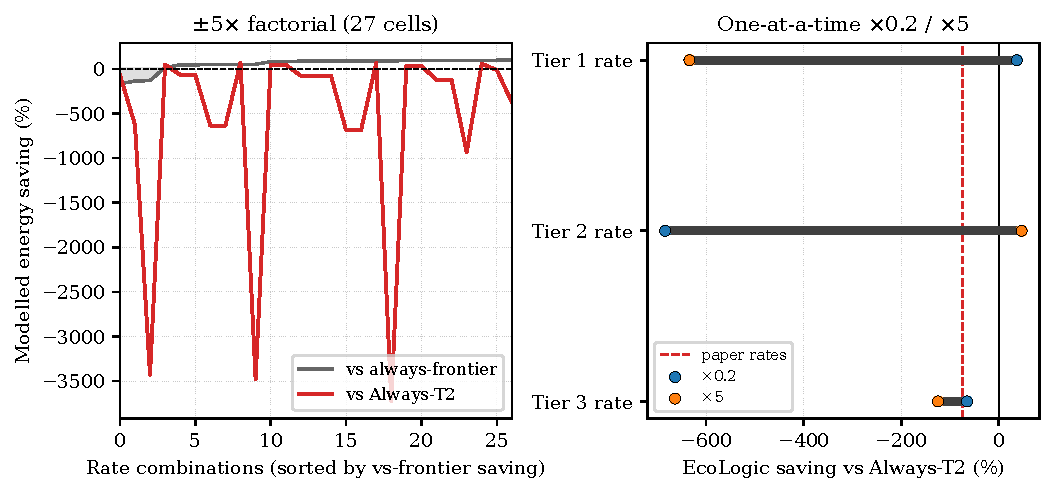
\includegraphics[width=\columnwidth]{fig_sensitivity.pdf}
\caption{Left: modelled energy saving of EcoLogic versus always-frontier (grey) and versus Always-T2 (red) across all $27$ rate combinations, sorted by the versus-frontier value. Zero is a sign change. Shading marks versus-frontier losses. Right: one-at-a-time $\times0.2$/$\times5$ tornado of the Always-T2 gap. All quantities are token-linear modelled joules.}
\label{fig:sens}
\end{figure}

\begin{table}[t]
\caption{$\pm5\times$ energy-model factorial ($27$ cells) and structured alternatives. Savings are EcoLogic versus the named baseline.}
\label{tab:sens}
\centering
\begin{tabular}{lr}
\toprule
Quantity & Value \\
\midrule
vs frontier, paper rates & $+88.6\%$ \\
vs frontier, band & $[-164.6\%,+98.8\%]$ \\
vs frontier, sign flips & $3/27$ \\
vs Always-T2, paper rates & $-74.9\%$ (router uses more) \\
vs Always-T2, EcoLogic cheaper & $8/27$ cells \\
Substitute rates $1.1/2.0/60$ & Eco $1380$\,J / T2 $525$\,J \\
\bottomrule
\end{tabular}
\end{table}

\subsection{Joules versus dollars as a reporting failure}

Table~\ref{tab:axes} prices the \emph{same} EcoLogic and always-frontier assignments two ways. Modelled joules say EcoLogic costs $0.114\times$ the frontier ($88.6\%$ saving). Measured USD say $0.450\times$ ($55.0\%$ saving). Residual cost moves by $0.450/0.114\approx3.97$---the ``roughly $4\times$'' gap flagged in the evaluation corpus. Always-T2 is even more flattering on USD ($0.066\times$ frontier) than on joules ($0.065\times$), because Together prices for \texttt{gpt-oss-20b} are far below OpenAI's \texttt{gpt-4o} prices, while the assumed J/1k ratio ($60/1.5=40$) is a different story than the dollar ratio.

This is a green-measurement result, not an accounting curiosity. Organisations that report ``energy saved versus GPT-4o'' using token-linear intensities will publish a larger success than the invoice shows, or the reverse, depending on how they set $r_t$. Neither axis is ``the true joule.'' Only USD was observed. The honest statement is: \emph{choice of cost model moves the headline by a factor of four on identical routing decisions, and both headlines are still the wrong comparison until Always-T2 is in the table.}

\begin{table}[t]
\caption{Two cost axes, identical assignments. USD from stored provider usage; joules from the linear token model.}
\label{tab:axes}
\centering
\begin{tabular}{lrrr}
\toprule
Policy & Modelled J & USD & vs T3 (J / \$) \\
\midrule
EcoLogic & $689$ & $\$0.2867$ & $0.114\times$ / $0.450\times$ \\
Always-T2 & $394$ & $\$0.0418$ & $0.065\times$ / $0.066\times$ \\
Always-T1 & $677$ & $\$0.3342$ & $0.112\times$ / $0.525\times$ \\
Frontier & $6066$ & $\$0.6366$ & $1$ / $1$ \\
\bottomrule
\end{tabular}
\end{table}

\section{Implications for Green Software Engineering}

\subsection{Metrics that always-frontier can game}

A sustainability metric that scores a system against ``the most expensive plausible default'' will certify almost any filter that drops expensive calls. EcoLogic's UI quantity \texttt{energy\_saved} versus a $500$\,J/1k GPT-5 ghost is an extreme instance; versus-\texttt{gpt-4o} at $88.6\%$ is the respectable instance. Both fail Lago et al.'s demand that sustainability claims be properties of the software, not of an unexamined alternative~\cite{lago2015framing}. The minimum non-gameable control set for a $k$-tier router is the $k$ static single-tier policies plus an oracle (to separate pool headroom from dispatcher quality). Random assignment is a useful additional floor: EcoLogic loses to it on accuracy ($86.8\%$ vs.\ $90.7\%$) because it systematically avoids the two better tiers.

\subsection{Architecture: discover a dominating static tier first}

Query-conditioned escalation is a reasonable tactic when (i)~tiers are quality-ordered, (ii)~the expensive tier is rarely needed, and (iii)~the cheap tier is actually cheap \emph{per query}, not merely per token. On this object none of the three hold: Tier~2 matches or beats the frontier, the classifier still spends most tokens on a verbose ``cheap'' tier, and three frontier calls add joules without adding correctness. The resulting architecture---a heuristic dispatcher in front of a heterogeneous pool---is then a sustainability anti-pattern in the sense of Capilla et al.~\cite{capilla2024architecture}: an extra component whose runtime effect is more energy and worse quality.

The design implication is operational. Before introducing a router, measure static single-tier energy$\times$quality on a representative, objectively graded sample. If one tier Pareto-dominates the others, ship that tier. A router is justified only when it traces a better frontier than every constant. That test is cheaper than building the router.

Cruz and Abreu catalogued energy \emph{patterns} for mobile applications---repeatable design decisions with a signed energy effect~\cite{cruz2021energy}. Query-conditioned LLM escalation is a candidate pattern with an unsigned effect: it saves energy when the cheap model is both good enough and actually cheap per request, and wastes energy when those premises fail. EcoLogic is an instance of the failure mode. Publishing it as a named anti-pattern (``escalate-past-a-dominating-tier'') is more useful to GREENS than another $88\%$ dashboard number.

GREENS frames sustainability in four dimensions---economic, social, environmental, and technical---with trade-offs~\cite{lago2015framing}. On this object the dimensions do not trade: Always-T2 is cheaper in USD, higher quality (a social/technical property for end users), and lower modelled energy. The router is not a compromise; it is dominated on the three dimensions we can score. That is unusual and worth stating, because many green tactics \emph{do} buy environmental gain with a quality or cost tax. Here there is no tax to justify the dispatcher.

\subsection{Report the energy model as part of the result}

Henderson et al.\ and Dodge et al.\ argued for systematic energy/carbon reporting in ML~\cite{henderson2020towards,dodge2022measuring}. For LLM serving, the analogous requirement is to publish (a)~whether joules were metered or modelled, (b)~the functional form and every constant, (c)~a $\pm$factor sweep on those constants, and (d)~the same table in at least one rate-independent unit (here, USD). Token-linear models are acceptable as \emph{scenarios}; they are not measurements. GREENS's interest in metrics for sustainability-aware SE is not served by scenarios presented as observations.

A practical checklist for a $k$-tier generative system follows (Table~\ref{tab:check}). Name the functional unit (we use ``graded item,'' not ``ChatGPT-equivalent query''). Include all $k$ static policies. State the energy model in one equation. Sweep the constants. Cross-tabulate a second axis that does not use those constants. If the ranking versus the cheapest competent static policy is unstable, do not ship a green claim. EcoLogic fails that checklist twice: the ranking versus Always-T2 is unfavourable at the system's own rates, and the ranking versus the frontier is unstable in the $\pm5\times$ cube.

\begin{table}[t]
\caption{Minimum non-gameable energy report for a $k$-tier LLM serving system. GREENS's interest is the metric, not a new model.}
\label{tab:check}
\centering
\setlength{\tabcolsep}{3pt}
\begin{tabular}{lp{0.62\columnwidth}}
\toprule
Item & Requirement \\
\midrule
Metering & Metered watts \emph{or} explicit token-linear model with every $r_t$. \\
Functional unit & Graded item vs.\ cheapest competent static policy, not vs.\ ghost frontier. \\
Static pool & All $k$ always-tier policies $+$ oracle (pool vs.\ dispatcher). \\
Sensitivity & Factorial on unsourced constants; report sign flips. \\
Second axis & Same assignments in a rate-independent unit (here, USD). \\
Surface & Lock raw vs.\ wrapped (or equivalent) before seeing energy. \\
\bottomrule
\end{tabular}
\end{table}

We do not argue that dollars are a better \emph{environmental} metric than joules. Invoices omit PUE, water, and idle capacity~\cite{wu2022sustainable,luccioni2024power}. We argue only that when joules are a linear restatement of tokens, publishing them as ``energy saved'' without the static-pool table is a green-software reporting failure---the same class of failure Naumann et al.\ designed GREENSOFT to prevent~\cite{naumann2011greensoft}.

\section{Threats to Validity}
\label{sec:threats}

\paragraph{Unmetered joules (primary).}
Not one joule in this paper was measured. A hostile reading is the correct one: we multiplied tokens by constants from \texttt{backend/main.py} that have no cited derivation, no hardware, and no utilisation. The $\pm5\times$ sweep bounds sensitivity to those three numbers. It does not validate linearity, ignore idle power, or substitute for a wattmeter on known GPUs~\cite{samsi2023words,luccioni2024power}. If real $r_t$ differ by more than $5\times$, or if energy is not proportional to tokens (batching, prefix caching, speculative decoding), every ranking that depends on $r$ can move. Rankings that do \emph{not} depend on $r$ still stand: Always-T2's accuracy dominance, the $11.5\times$ token inflation, and the USD table.

\paragraph{Substitute models.}
Gemma~3N~E4B and Apriel~1.6~15B were retired. Qwen3.5-9B and \texttt{gpt-oss-20b} are larger reasoning models. The $11.5\times$ token penalty is likely substitution, not EcoLogic's intended stack. We characterise the routing policy faithfully and the original lineup only by analogy. A metered rerun on the original slugs is impossible from this repository.

\paragraph{In-sample keyword router and $n=364$.}
The classifier is a fixed heuristic evaluated on the item set it was not trained on but also not held out from in a pre-registered sense. Keyword rules can overfit a developer's intuition about ``what looks like code.'' Prompt surface form is a further stability threat: wrapping items in benchmark instructions (``Complete the following Python function...'') changes the assigned tier on $47\%$ of items and multiplies modelled energy from $689$\,J to $3419$\,J, largely by escalating HumanEval to Tier~3. We report raw-query routing because that is what a user types; it is also the choice more favourable to the router. Sample size $364$ is small for rare-escalation behaviour ($3$ frontier calls). Wilson intervals capture item sampling, not generation noise; a temperature-$0$ repeat on $21$ items moved completion tokens by tens of percent on the reasoning tiers (mean absolute per-item moves of $20\%$ / $30\%$ / $1.5\%$ on Tiers~1/2/3), so energy totals have additional run-to-run uncertainty. Benchmarks are public, single-turn, and almost certainly in training data; absolute accuracies are optimistic. Real EcoLogic traffic was not sampled. The $45\%$/$27\%$/$27\%$ HumanEval/MMLU/GSM8K mix is a specification artifact, not a measured production distribution; any other mix would reweight Table~\ref{tab:bench}.

A learned replacement router, trained under a held-out protocol on a larger pool, is outside this paper's identity. For bounding: it did not beat Always-T2 on quality. We do not use that result as a main experiment.

\paragraph{Oracle and Always-T2 selection.}
The oracle overfits a single generation. Always-T2 is the best constant \emph{after} seeing the table. As a control that a router must beat, that is intended. As a claim that operators would have known to ship Tier~2 \emph{a priori}, it is not: discovering the dominating static tier is itself an evaluation cost, albeit a smaller one than operating a mis-calibrated dispatcher forever. On a different mix---for example, a production workload where the frontier is actually a quality ceiling---the anti-pattern reading would not apply. We did not observe that mix.

We mention only for completeness that an external two-model router, RouteLLM, has been reported to pass a cost-matched static mixture on its own GSM8K release with a sub-point effect; that is a different system, a different axis, and not a result of this paper.

\paragraph{What a metered follow-up would have to do.}
A hostile reviewer who accepts the architecture argument but rejects every joule number is right to demand wall power. The next measurement, which this repository cannot supply, is: known GPUs, known batch size, power at the wall or from NVML/RAPL with a documented idle baseline, the original (or current) serving slugs, and a traffic mix sampled from production rather than HumanEval. Until that exists, EcoLogic's \texttt{energy\_saved} field should be treated as a UX quantity, not as an environmental KPI. The ranking on \emph{tokens} and on \emph{USD} does not wait on that meter: Always-T2 uses $4.4\times$ fewer tokens and $6.87\times$ fewer dollars than EcoLogic at higher accuracy.

\section{Conclusion}

EcoLogic advertises energy saved against a frontier default. Under its own token-linear energy model, a policy that ignores the query and always calls the middle tier is $5.5$\,pp more accurate at $0.57\times$ the modelled joules. The $88.6\%$ versus-frontier joule headline is the wrong comparison, is not a wattmeter reading, is not sign-stable under a $\pm5\times$ rate sweep, and disagrees by a factor of four with measured dollars on the same assignments.

For green software engineering the lesson is architectural and metrological. Do not certify a router against always-frontier. Put the static pool on the plot first. Prefer discovering a dominating static tier before adding a dispatcher. When you must model energy as tokens times a rate, publish the rates, sweep them, and never treat the product as observed joules. EcoLogic is one deployed counter-example; the metric failure it exhibits---baseline gaming plus an unmetered linear proxy---is available to any generative-AI system that ships a green dashboard.

\section*{Data}
All numbers reconstruct from committed \texttt{raw\_results/} via \texttt{papers/greens/analysis.py}. No new model calls were made for this manuscript.

\bibliographystyle{IEEEtran}
\bibliography{refs}

\end{document}
